\chapter{Evaluation}
This chapter shall present the results of my study and discuss the implications of what was observed.

The performance of \acrshort{abe} greatly depends on the underlying implementation of the elliptic curves and pairing because those are the most expensive operations performed by the schemes presented in Chapter~\ref{chapter:constructions}.
Therefore, the performance of the ported \texttt{rabe-bn} library will be evaluated in Section~\ref{sec:rabebn-evaluation} before turning to the performance of the actual \acrshortpl{abes} in Section~\ref{sec:abe-performance}.

\section{Performance of \texttt{rabe\_bn}}\label{sec:rabebn-evaluation}

See Table~\ref{tbl:rabebn-performance} for performance measurements of random element sampling, group-scalar exponentiation and the pairing operation.
The times have been measured using randomly sampled elements and averaged over 100 calls each.

% TODO maybe evaluate RAM usage of these operations?
\begin{center}
    \begin{tabular}{|c|r|r|}\hline%
        Operation & SoC [ms] & Laptop [ms]\\\hline\hline
        \csvreader[late after line=\\]%
        {data/bn-smpl.csv}{op=\op,soc=\soc,laptop=\laptop}%
        {\op&\soc&\laptop}%
        % \hline
        % \csvreader[late after line=\\]%
        % {data/bn-groupop.csv}{op=\op,soc=\soc,laptop=\laptop}%
        % {\op&\soc&\laptop}%
        \hline
        \csvreader[late after line=\\]%
        {data/bn-groupexp.csv}{op=\op,soc=\soc,laptop=\laptop}%
        {\op&\soc&\laptop}%
        \hline
        \csvreader[late after line=\\]%
        {data/bn-pairing.csv}{op=\op,soc=\soc,laptop=\laptop}%
        {\op&\soc&\laptop}%
        \hline
    \end{tabular}  
    \captionof{table}{Execution times for various operations on the SoC and the laptop}
    \label{tbl:rabebn-performance}
\end{center}


It is evident that the the cost of the operations differs greatly between the groups. 
Sampling a random element takes about the same time as group exponentiation for $\mathbb{G}_1$ and $\mathbb{G}_2$, but is significantly more costly for $\mathbb{G}_T$.
Looking at the implementation, the reason for this is obvious: Sampling from $\mathbb{G}_1$ and $\mathbb{G}_2$ simply generates a random $z \in \mathbb{F}_r$ and returns the group element $z \cdot G$ for $G$ a generator.
Sampling from $\mathbb{G}_T$ is done by generating random elements of $\mathbb{G}_1$ and $\mathbb{G}_2$ and computing their pairing.
This is reflected in the measured timings.

Interestingly, RAM size seems to be a limiting factor when computing pairings on embedded devices.
During development, I also tested the ported \texttt{rabe-bn} library on the nRF52832 SoC, which has 64\,KB of RAM (vs. 256\,KB in the nRF52840). 
On this chip, a pairing could be computed successfully only if the library was built \emph{without debug symbols}.
With debug symbols, there was not enough RAM available and the pairing computation failed.
This suggests that the memory use during pairing computation is close to 64\,KB, which would still be a quarter of the RAM on the nRF52840 SoC.
While this memory is not consumed permanently, it still needs to be available when the pairing function is called.

Measurement of the RAM use with Valgrind on the laptop shows that one pairing computation needs 58,552\,KB of RAM.
This is indeed close to the 64\,KB and thus supports our assumption that RAM use on the laptop is representative for RAM use on the SoC.

\section{Evaluation of the ABE library}\label{sec:abe-performance}

In this section, the performance of the four algorithms Encrypt, Decrypt, Setup and KeyGen of the two \acrshort{abe} schemes GPSW and YCT will be evaluated.

For the results of the runtime analysis, see Figures~\ref{fig:abe-performance-diagrams-gpsw} and \ref{fig:abe-performance-diagrams-yct}. 
For the analysis of RAM use, see Figure~\ref{fig:abe-performance-diagrams-ram}; for flash use see Figure~\ref{fig:abe-performance-diagrams-flash}. 


\subsection{Methods of measurement}
This section describes how the presented result were obtained.

\subsubsection{Time measurements}
\begin{figure}[h]\centering
    \begin{subfigure}[h]{0.45\textwidth}
        \begin{tikzpicture}
            \begin{axis}[
                title={Timing of GPSW \cite{goyal_attribute-based_2006} on the SoC},
                xlabel={attributes / leaf nodes},
                ylabel={seconds},
                xmin=0, xmax=32,
                ymin=0, ymax=81000000,
                scaled y ticks=base 10:-6,
                ytick scale label code/.code={}, % removes the '\cdot 10^3' label 
                legend pos=north west,
                grid=major,
                grid style=dashed,
                legend style={nodes={scale=0.65, transform shape}}
            ]
            \addlegendentry{Setup};
            \addplot [color=orange, mark=square] table [x=atts,y=setup,col sep=comma] {data/gpsw06-soc.csv};
            \addlegendentry{Encrypt};
            \addplot [color=blue, mark=triangle] table [x=atts,y=enc,col sep=comma] {data/gpsw06-soc.csv};
            \addlegendentry{KeyGen};
            \addplot [color=green, mark=o] table [x=atts,y=keygen,col sep=comma] {data/gpsw06-soc.csv};
            \addlegendentry{Decrypt};
            \addplot [color=red, mark=+] table [x=atts,y=dec,col sep=comma] {data/gpsw06-soc.csv};
            \end{axis}
        \end{tikzpicture}
    \end{subfigure}%
    \hspace{0.09\textwidth}
    \begin{subfigure}[h]{0.45\textwidth}
        \begin{tikzpicture}
            \begin{axis}[
                title={Timing of YCT \cite{yao_lightweight_2015} on the SoC},
                xlabel={attributes / leaf nodes},
                ylabel={seconds},
                xmin=0, xmax=32,
                ymin=0, ymax=11500000,
                scaled y ticks=base 10:-6,
                ytick scale label code/.code={}, % removes the '\cdot 10^3' label 
                legend pos=north west,
                grid=major,
                grid style=dashed,
                legend style={nodes={scale=0.65, transform shape}}
            ]
            \addlegendentry{Setup};
            \addplot [color=orange, mark=square] table [x=atts,y=setup,col sep=comma] {data/yct14-soc.csv};
            \addlegendentry{Encrypt};
            \addplot [color=blue, mark=triangle] table [x=atts,y=enc,col sep=comma] {data/yct14-soc.csv};
            \addlegendentry{KeyGen};
            \addplot [color=green, mark=o] table [x=atts,y=keygen,col sep=comma] {data/yct14-soc.csv};
            \addlegendentry{Decrypt};
            \addplot [color=red, mark=+] table [x=atts,y=dec,col sep=comma] {data/yct14-soc.csv};
            \end{axis}
        \end{tikzpicture}
    \end{subfigure}%
    % \caption{Performance of GPSW and YCT on the SoC.}
    \vspace{1cm}
    \begin{subfigure}[h]{0.448\textwidth}
        \begin{tikzpicture}
            \begin{axis}[
                title={Timing of GPSW \cite{goyal_attribute-based_2006} on the laptop},
                xlabel={attributes / leaf nodes},
                ylabel={milliseconds},
                xmin=0, xmax=32,
                ymin=0, ymax=301000,
                scaled y ticks=base 10:-3,
                ytick scale label code/.code={}, % removes the '\cdot 10^3' label 
                legend pos=north west,
                grid=major,
                grid style=dashed,
                legend style={nodes={scale=0.65, transform shape}}
            ]
            \addlegendentry{Setup};
            \addplot [color=orange, mark=square] table [x=atts,y=setup,col sep=comma] {data/gpsw06-laptop.csv};
            \addlegendentry{Encrypt};
            \addplot [color=blue, mark=triangle] table [x=atts,y=enc,col sep=comma] {data/gpsw06-laptop.csv};
            \addlegendentry{KeyGen};
            \addplot [color=green, mark=o] table [x=atts,y=keygen,col sep=comma] {data/gpsw06-laptop.csv};
            \addlegendentry{Decrypt};
            \addplot [color=red, mark=+] table [x=atts,y=dec,col sep=comma] {data/gpsw06-laptop.csv};
            % \addplot [color=black, mark=+] table [x=atts,y=dec2,col sep=comma] {data/gpsw06-laptop.csv};
            % \addplot [color=olive, mark=+] table [x=atts,y=dec3,col sep=comma] {data/gpsw06-laptop.csv};
            \end{axis}
        \end{tikzpicture}
    \end{subfigure}
    \hspace{0.09\textwidth}
    \begin{subfigure}[h]{0.448\textwidth}
        \begin{tikzpicture}
            \begin{axis}[
                title={Timing of YCT \cite{yao_lightweight_2015} on the laptop},
                xlabel={attributes / leaf nodes},
                ylabel={milliseconds},
                xmin=0, xmax=32,
                ymin=0, ymax=110000,
                scaled y ticks=base 10:-3,
                ytick scale label code/.code={}, % removes the '\cdot 10^3' label 
                legend pos=north west, 
                grid=major,
                grid style=dashed,
                legend style={nodes={scale=0.65, transform shape}}
            ]
            \addlegendentry{Setup};
            \addplot [color=orange, mark=square] table [x=atts,y=setup,col sep=comma] {data/yct14-laptop.csv};
            \addlegendentry{Encrypt};
            \addplot [color=blue, mark=triangle] table [x=atts,y=enc,col sep=comma] {data/yct14-laptop.csv};
            \addlegendentry{KeyGen};
            \addplot [color=green, mark=o] table [x=atts,y=keygen,col sep=comma] {data/yct14-laptop.csv};
            \addlegendentry{Decrypt};
            \addplot [color=red, mark=+] table [x=atts,y=dec,col sep=comma] {data/yct14-laptop.csv};
            % \addlegendentry{Decrypt};
            % \addplot [color=black, mark=+] table [x=atts,y=dec2,col sep=comma] {data/yct14-laptop.csv};
            % \addplot [color=olive, mark=+] table [x=atts,y=dec3,col sep=comma] {data/yct14-laptop.csv};
            % \addplot [color=green, mark=+] table [x=atts,y=dec4,col sep=comma] {data/yct14-laptop.csv};
            \end{axis}
        \end{tikzpicture}
    \end{subfigure} 
    \caption[Performance of ABE schemes on the SoC and laptop]{Performance of GPSW and YCT on the SoC and on the laptop. Note the different scales between the SoC and the laptop (seconds vs. milliseconds!)}
    \label{fig:abe-performance-diagrams}
\end{figure}

All times were measured using a hardware timer on the nRF52840 SoC.

For Setup, the number of attributes refers to the total number of attributes in the system.
For Encrypt, the number of attributes refers to the number of attributes under which a ciphertext is encrypted.

For KeyGen, the number of attributes refers to the number of leaf nodes in the used access policy.
The \glspl{access-tree} consists only of a root node and the given number of children, i.e. the root node has up to 30 children. 
To ensure that all leaves have to be evaluated, the threshold is set to the number of children (the root acts as an \emph{AND} node).
This approach is also found in other evaluations of \acrshort{abe}~\cite{girgenti_feasibility_2019}.

For Decrypt, the same access policies from KeyGen are used to decrypt a ciphertext encrypted with all system attributes.
This ensures that the ciphertext can always be decrypted, and does not influence the decryption speed.

For reference, the same measurements were made on the laptop.
These timings are included in Appendix~\ref{sec:appendix_laptop}.

\subsubsection{RAM use measurements}
\begin{minipage}{\textwidth}\centering
    \begin{tikzpicture}
        \begin{axis}[
            % title={RAM use during decryption},
            height=.7\textheight,
            xlabel={depth of the \gls{access-tree}},
            ylabel={kilobytes},
            xmin=0.75, xmax=4.25,
            ymin=0, ymax=360000,
            xtick=data,
            scaled y ticks=base 10:-3,
            ytick scale label code/.code={}, % removes the '\cdot 10^3' label 
            legend pos=north west,
            grid=major,
            minor y tick num=1,
            grid style=dashed,
            legend style={nodes={scale=.8, transform shape}}
        ]
        \addlegendentry{GPSW Dec};
        \addplot [color=blue, mark=o] table [x=layers,y=gpsw-dec,col sep=comma] {../thesis/data/ram.csv};
        \addlegendentry{YCT Dec};
        \addplot [color=orange, mark=triangle] table [x=layers,y=yct-dec,col sep=comma] {../thesis/data/ram.csv};
        \addlegendentry{GPSW Enc};
        \addplot [color=blue, mark=none] {83560};
        \addlegendentry{YCT Enc};
        \addplot [color=orange, mark=none] {22616};
        \addplot [color=black, dashed, mark=none] {256000};
    \end{axis}
    \end{tikzpicture}
\end{minipage}

RAM use is not presented for encryption and key generation because those algorithms use a constant amount of memory.
The RAM use of key generation and decryption depends only on the depth of the access tree.
For this reason, the flat policies from the timing evaluation could not be re-used for RAM evaluation.
Instead, \glspl{access-tree} in the shape of \glspl{perfect-binary-tree} were employed.

The values were obtained by running decryption on the laptop and measuring the RAM use using Valgrind's \texttt{Massif} tool~\cite{nethercote_massif_nodate}.
Valgrind is a tool suite for analyzing memory use and memory management of programs.
Massif itself is originally a heap profiler, but can also be used to measure the stack's memory use with the option \verb+--stacks=yes+.
Heap use is not profiled because our library is specifically written to work without the heap.

Massif outputs a number of measurements for different instants during the runtime of the program. 
The presented values represent the maximum stack memory use during the entire runtime.

It is assumed that RAM use on the laptop is representative for RAM use on the SoC.
This is in line with other evaluations of \acrshort{abe}~\cite{borgh_attribute-based_2016}. 
In addition, decryption with the same policies on the SoC confirmed this assumption:
With three- and four-layer policies, decryption failed on the SoC, but it worked with one- and two-layer policies.
The RAM use on the laptop is below 256\,KB (the RAM size of the SoC) for the two-layer policy, but above 256\,KB for the three-layer policy.

\subsubsection{Flash size measurements}
\begin{figure}[h]\centering
    \pgfplotsset{scaled y ticks=false}
    \begin{tikzpicture}
        \begin{axis}[
            ybar,
            bar shift=0pt,
            ylabel={kilobytes},
            title={Size of executable},
            width=0.7\textwidth,
            height=0.4\textheight,
            symbolic x coords={GPSW,YCT},
            xtick={GPSW,YCT},
            ymin=0, ymax=175,
            bar width=2cm,
            enlarge x limits = 0.75,
            nodes near coords,
            every node near coord/.style={
                /pgf/number format/precision=2
            },
        ]
        \addplot[blue, fill=blue!30] coordinates {
            (GPSW, 148.824)
        };
        \addplot[orange, fill=orange!30] coordinates {
            (YCT,	88.288)
        };
        % \addlegendentry{SoC RAM size};
        % \addplot [color=black, mark=none] {262144};
        \end{axis}
    \end{tikzpicture}
    \caption[Flash use of the ABE library executable]{Comparison of the flash size of the ABE library when using the two schemes.}
    \label{fig:abe-performance-diagrams-flash}
\end{figure}

The sizes of the executable binaries were measured by calling \verb+cargo size -- -A+ with optimizations on a binary crate that contains a minimal code snippet calling the respective \acrshort{abe} library.
\verb+cargo size+ is part of \verb+cargo-binutils+~\cite{noauthor_cargo-binutils_nodate}, which provides access to the LLVM tools in the Rust toolchain.
The presented sizes are the combined size of the \texttt{text}, \texttt{rodata} and \texttt{bss} segments.


\subsection{Results}
The pairing-free YCT scheme is significantly faster than the pairing-based GPSW scheme in all four algorithms. 
For both schemes, Setup takes about the same time as Encryption for the same number of attributes in the system or ciphertext, respectively.
The runtime of Setup and Encrypt with GPSW is about 3.5\,s longer than with YCT, independent on the number of attributes.
% On the SoC, setup and encryption with a single attribute take about 4 seconds with GPSW and only about 0.4 seconds with YCT.
% With 30 attributes, GPSW requires about 8.5 seconds and YCT about 5 seconds.
The runtimes increase linearly in both, with each additional attribute adding about 150\,ms.

For the KeyGen algorithm, difference is even larger:
The runtime of GPSW increases considerably with larger policies.
With a single-attribute policy, KeyGen takes about 650\,ms. With 25 attributes, it already takes more than 16 seconds.
The runtime of YCT only increases slightly from 35\,ms for one attribute to 210\,ms for 25 attributes.

Decryption time is also linear with both schemes.
Again, YCT is much faster than GSPW with YCT taking 12\,s and GPSW taking 80\,s for the largest policy.

The RAM use also shows a large advantage for YCT:
With GPSW, a single-level policy already uses up more than three times more RAM than YCT; this difference only increases with more policy levels.
With three or more levels, decryption fails entirely on the SoC because there is not enough RAM.
Assuming RAM use on the laptop is representative for the SoC, the single-level policy already requires more than two thirds of the total RAM on the sensor.
YCT does not have this problem: Even with a four-level policy, it uses only the equivalent of about a quarter of the total RAM.

The difference in flash size is not as big, but the GPSW scheme still requires about 70\,\% more flash storage than the YCT scheme.


\section{Discussion}
The timings of Setup and Encrypt are in line with the time-consuming operations performed by the algorithms: 
In both schemes, each additional attribute results in one additional exponentiation in $\mathbb{G}_1$.
This takes about 150\,ms as per Table~\ref{tbl:rabebn-performance}, which is exactly the additional time per attribute.
The constant overhead of about 3.5\,s with GPSW is a result of the pairing computation and exponentiation in $\mathbb{G}_T$ (for Setup) and the sampling and exponentiation in $\mathbb{G}_T$ (for Encrypt).

This contradicts the result from \cite{girgenti_feasibility_2019}, where the encryption performance of GPSW and YCT are explicitly noted to be equivalent.
However, their conclusion is based on very small numbers of attributes for YCT due to a bug in the evaluated library.
In addition, their SoC is significantly faster than ours (240\,MHz vs. 64\,MHz), thus the constant overhead of GPSW is smaller.

For the KeyGen algorithm, the speed difference between YCT and GSPW is especially striking: 
The YCT algorithm is extremely fast for a small number of attributes (below 100\,ms) and only increases slightly as more attributes are added.
GPSW is not only slower already for a few attributes, but its runtime also increases much more quickly when increasing the policy size.
Again, looking at the schemes, the reason becomes evident: YCT's KeyGen only works on elements of $\mathbb{F}_r$, which are small and easy to calculate with.
GPSW uses secret shares from $\mathbb{G}_2$, for which operations take considerably more time.
This is also the case for decryption: YCT only requires exponentation and point addition in $\mathbb{G}_1$, whereas GPSW performs pairings, multiplications and exponentiations in $\mathbb{G}_T$.

The RAM consumption of decryption with GPSW is a limiting factor on the SoC:
Decryption with policies of more than two layers fails because of too little memory.
Unlike the timing results, this poses a hard limit on the size of \glspl{access-policy}.
Also, in our evaluation, the \acrshort{abe} library was able to use all of the available RAM on the SoC.
In a real-world use case, the application employing \acrshort{abe} might already occupy a considerable portion of the available RAM, leaving too little space even for decryption with small \glspl{access-tree}.
This problem is much less pronounced with the pairing-free YCT scheme.

If some latency is acceptable, doing encryption with \acrshort{abe} on the SoC is feasible if the number of attributes is not very large.
The pairing-free YCT scheme performs better, but the pairing-free GPSW scheme is still good enough for encryption.

With decryption, the YCT scheme is to be preferred:
With GPSW, decryption takes considerably more time and uses a large amount of RAM.
This results in the mentioned hard limit on the policy depth, which is not present with YCT.

However, as the security of pairing-free \acrshort{abes} is questioned (see \cite{herranz_attacking_2020}), a pairing-based scheme might be preferable.
Therefore, in applications where only encryption is necessary on the SoC, the GPSW scheme might be preferred over YCT.

The other two algorithms, Setup and KeyGen, are run only by the \acrshort{kgc}.
Therefore, it is reasonable to assume that these don't need to be run on a constrained node in real-world scenarios.
The \acrshort{kgc} would probably be a specially protected PC or at least a powerful \acrshort{iot} node (e.g. Raspberry Pi).

\section{Further Improvements / Future Work}

The implementations evaluated in this thesis offer room for improvement in many ways.
For one, interoperability between the ``light'' \acrshort{abe} library presented here and a potential ``full'' counterpart (e.g. for the \acrshort{kgc}) was not a priority.

Regarding the results on the SoC, improvements could be made by improving the underlying pairing and elliptic curve implementation of the \texttt{rabe-bn} library.
Even though the operations remain computationally expensive, other implementations do significantly better:
In \cite{scott_deployment_2020}, the \emph{MIRACL Core} library was tested on the same SoC as ours using the same type of curve (256-bit BN curve).
This library evaluates a pairing in about 600\,ms; our library takes 1600\,ms. 
Exponentiation in $\mathbb{G}_T$ takes about 300\,ms with their library and about 1400\,ms with ours. 
Both libraries are high-level implementations (i.e. no optimized assembly code), and thus it is likely that the optimizations from \emph{MIRACL Core} could be carried over to Rust.
As the runtime of \acrshort{abe} is dominated by these expensive curve operations, an improved pairing and curve implementation offers considerable potential for speedup.
These improvements, however, are clearly outside the scope of this thesis.

Runtimes in the order of several seconds might still be too long, even if improved by a better pairing library.
To aid this, the symmetric key used to encrypt the actual payload may be reused:
In both implemented schemes, the data is not encrypted directly but rather using a hybrid approach, i.e. a random key is generated and encrypted under \acrshort{abe} (so-called key encapsulation).
This key is then used to encrypt the actual payload using AES (so-called data encapsulation).
This approach allows fast encryption and decryption of messages of arbitrary size and is standard practice with \glspl{pkes}.

Usually, a new key is generated and encrypted for every message, but this is not strictly necessary:
By saving both the symmetric key and its \acrshort{abe}-encrypted version, more than one message can be encrypted with the same symmetric key.
A single \acrshort{abe} encryption operation can then be used for many messages.
The encyptor may periodically generate and encrypt a new symmetric key (e.g. once per day).
If the messages should be decryptable on their own, the \acrshort{abe}-encrypted symmetric key can be copied into each encrypted message.
The downside is that all messages encrypted with the same symmetric key naturally have the same attributes or access policy attached (i.e. reduced granularity).
Also, if the symmetric key is compromised (possibly while it is stored to encrypt the next message), all messages encrypted with that key will be compromised.

This approach does not reduce the ciphertext size because the \acrshort{abe}-encrypted key is copied into each ciphertext.
If this is an issue (e.g. due to low-power wireless transmission), the \acrshort{abe}-encrypted key may be transmitted separately from the symmetrically encrypted messages.
Then, both the symmetric ciphertext of and the respective \acrshort{abe}-encrypted key must be present to decrypt a message.

This symmetric key-caching approach was implemented for use in a system similar to that presented in Figure~\ref{fig:system-architecture}.
However, it was not evaluated for this thesis, because it doesn't represent ``true'' \acrlong{abe}.
~\\

The two schemes implemented in the library are \acrshort{kp-abe} schemes, currently no \acrshort{cp-abe} schemes are implemented.
The implemented schemes also don't support key revocation, key delegation or a \gls{large-universe} of attributes. 
Implementation and evaluation of such schemes is left for future projects.
